\chapter{Caractéristiques des ondes mécaniques}
\section{Principe de superposition des ondes}
Quand deux ondes ou plus passent en même temps par une même région de l'espace, on observe que le déplacement réel est la somme vectorielle des déplacements causés par chaque onde individuelle.
C'est le \motcle{principe de superposition des ondes}.
Les illustrations ci-dessous présentent respectivement deux ondes puis la superposition de celles-ci.
\begin{figure}[h]
    \begin{tikzpicture}
        \definecolor{olivegreen}{RGB} {0,125,15}
        \tikzset{>=latex}
        \tkzInit[xmin=-4,xmax=8,ymin=-1,ymax=1.5,xstep=1,ystep=1]
        \tkzDrawX[label={$X [m]$},below left=25pt]
        \tkzDrawY[label={$Y [m]$},right=5pt]
        \tkzAxeXY[label={}] %This macro combines the four macros: \tkzDrawX\tkzDrawY \tkzLabelX\tkzLabelYnode font=\tiny]
        \tkzFct[domain=-4:8,red]{sin(pi*x)}
    \end{tikzpicture}
    %\label{Une onde dont l'équation de l'élongation est donnée par \(y(t)=sin( \pi \cdot t) \)}
    \caption{Une onde dont l'équation de l'élongation est donnée par \(y(t)=sin( \pi \cdot t) \)}
\end{figure}

\begin{figure}[h]
    \begin{tikzpicture}
        \definecolor{olivegreen}{RGB} {0,125,15}
        \tikzset{>=latex}
        \tkzInit[xmin=-4,xmax=8,ymin=-1,ymax=1.5,xstep=1,ystep=1]
        \tkzDrawX[label={$X [m]$},below left=25pt]
        \tkzDrawY[label={$Y [m]$},right=5pt]
        \tkzAxeXY[label={}] %This macro combines the four macros: \tkzDrawX\tkzDrawY \tkzLabelX\tkzLabelYnode font=\tiny]
        \tkzFct[domain=-4:8,red]{sin(2*pi*x)}
    \end{tikzpicture}
    %\label{Une onde dont l'équation de l'élongation est donnée par \(y(t)=sin( \pi \cdot t) \)}
    \caption{Une onde dont l'équation de l'élongation est donnée par \(y(t)=sin(2 \cdot \pi \cdot t) \)}
\end{figure}

\begin{figure}[h]
    \begin{tikzpicture}
        \definecolor{olivegreen}{RGB} {0,125,15}
        \tikzset{>=latex}
        \tkzInit[xmin=-4,xmax=8,ymin=-2,ymax=2.5,xstep=1,ystep=1]
        \tkzDrawX[label={$X [m]$},below left=25pt]
        \tkzDrawY[label={$Y [m]$},right=5pt]
        \tkzAxeXY[label={}] %This macro combines the four macros: \tkzDrawX\tkzDrawY \tkzLabelX\tkzLabelYnode font=\tiny]
        \tkzFct[domain=-4:8,red]{sin(2*pi*x)+sin(pi*x)}
    \end{tikzpicture}
    %\label{Une onde dont l'équation de l'élongation est donnée par \(y(t)=sin( \pi \cdot t) \)}
    \caption{Une onde dont l'équation de l'élongation est donnée par \(y(t)=sin( \pi \cdot t)+sin(2 \cdot \pi \cdot t) \)}
\end{figure}

\newpage

Ce principe de superposition n'est valable que lorsque les élongations ne sont pas trop importantes et lorsque la force de rappel est proportionnelle au déplacement.
L'onde résultante n'est pas une onde sinusoïdale simple, on parle dans ce cas d'\motcle{onde composite}. On peut démontrer que toute onde composite peut être considérée comme étant composée de plusieurs ondes sinusoïdales simples de fréquence et amplitudes différentes. Ce concept a été introduit par Joseph Fourier en 1822. L'ensemble des ondes qui se combinent pour former une onde composite est appelé \motcle{série de Fourier}.
Les ondes simples qui se combinent pour former l'onde composite sont appelées \motcle{harmoniques} de l'onde. L'harmonique de plus petite fréquence, et dont les autres ne sont qu'un multiple, est appelée \motcle{harmonique fondamentale}.
Les séries de Fourier se rencontrent dans la décomposition de signaux périodiques, dans l'étude des courants électriques, des ondes cérébrales, dans la synthèse sonore, le traitement d'images, etc.
\newpage

\begin{figure}[h]
    \centering
    \includegraphics[width=.4\linewidth]{serie_fourier.png}
    \caption{Les quatre premières sommes partielles de la série de Fourier pour un signal carré.}
\end{figure}

\newpage

\section{Réflexion des ondes}
Lorsqu'une onde rencontre un obstacle ou qu'elle arrive à la fin du milieu dans lequel elle se propage, elle est au moins partiellement réfléchie.
Une onde ne se réfléchi pas de la même manière selon que l'extrémité du milieu soit fixe ou mobile.
\begin{figure}[h]
    \begin{minipage}{.5\textwidth}
        \centering
        \includegraphics[width=.8 \linewidth]{reflexion_fixee.png}
        \caption{Réflexion d'une onde dont l'extrémité est fixée.}
    \end{minipage}
    \begin{minipage}{.5\textwidth}
        \centering
        \includegraphics[width=.8 \linewidth]{reflexion_libre.png}
        \caption{Réflexion d'une onde dont l'extrémité est libre.}
    \end{minipage}
\end{figure}
On observe que lorsque l'extrémité est fixée, l'onde réfléchie est inversée ce qui n'est pas le cas lorsque l'extrémité est libre. Cela s'explique, car lorsque l'onde atteint l'extrémité fixée, elle exerce une force vers le haut sur le support qui, en retour, exerce une force réciproque vers le bas sur le support de l'onde (la corde ou autre chose).
Dans le cas d'une onde à deux ou trois dimensions, comme les vagues sur l'eau, il importe de considérer le \motcle{front} de l'onde, c'est-à-dire toute la largeur de la crête de l'onde, la ligne formée par tous les points oscillant en phase.
On appelle \motcle{rayon}, toute ligne de même direction que le déplacement de l'onde et perpendiculaire au front de celle-ci.

\newpage

\subsection{Loi de la reflexion}
Lorsqu'une onde est réfléchie sur une surface, l'angle d'incidence est égal à l'angle de réflexion. Ces deux angles, sont ceux entre le rayon de l'onde et la perpendiculaire à la surface de réflexion.
\begin{encadre}
    \(\theta_i = \theta_r\)
\end{encadre}

\begin{tikzpicture}[line cap=round,line join=round,>=triangle 45,x=1cm,y=1cm,use optics]
    \fill[line width=0pt,color=Brown,fill=Brown,pattern=north east lines,pattern color=Brown] (6,0)--(6,7)-- (7,7)-- (7,0)-- cycle;

    \tkzDefPoints{0/0/A,6/3.5/B,0/7/C,0/3.5/D}
    \tkzMarkAngle[mark=solid,-,color=ForestGreen](D,B,A)
    \tkzFillAngle[color=ForestGreen,fill=ForestGreen,fill opacity=0.1](D,B,A)
    \tkzLabelAngle[pos=1.5,color=ForestGreen](D,B,A){\(\theta _i\)}

    \tkzMarkAngle[mark=solid,-,color=ForestGreen](C,B,D)
    \tkzFillAngle[color=ForestGreen,fill=ForestGreen,fill opacity=0.1](C,B,D)
    \tkzLabelAngle[pos=1.5,color=ForestGreen](C,B,D){\(\theta _r\)}

    \draw [line width=1pt,color=black] (6,0)-- (6,7);
    \draw [->-,line width=1pt,color=red] (0,0) -- (6,3.5);
    \draw [-<-,line width=1pt,color=blue] (0,7)--(6,3.5);
    \draw [line width=1pt,color=LimeGreen] (0,3.5) -- (6,3.5);
    \begin{scriptsize}
        \draw [fill=black] (6,3.5) circle (2pt);
        \draw[color=LimeGreen] (3,4) node {n};
    \end{scriptsize}
\end{tikzpicture}

Lors de la réflexion, une partie de l'énergie mécanique est absorbée et transformée en chaleur. L'onde réfléchie aura donc une amplitude moindre que l'onde incidente.

\newpage

\section{Réfraction des ondes}
Quand une onde quelconque rencontre une frontière entre deux milieux, une partie de son énergie est réfléchie, une autre est absorbée et une dernière partie est transmise.
Lorsqu'une onde en deux ou trois dimensions traverse la frontière séparant deux milieux dans lesquels la vitesse de propagation n'est pas la même, l'onde transmise va changer de direction ; ce phénomène s'appelle la réfraction.
Une analogie peut être faite avec une ligne de soldats qui pénètre progressivement sur un terrain dans lequel elle avance moins vite. La ligne des soldats est alors progressivement infléchie et lorsqu'ils seront tous passés dans le deuxième terrain, le front de leur déplacement ne sera plus parallèle à celui qu'ils avaient avant.

\begin{figure}[h]
    \centering
    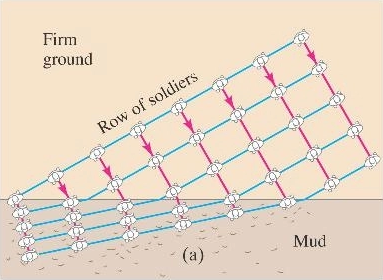
\includegraphics[width=.4\linewidth]{refraction_soldats.png}
    \caption{La réfraction d'une ligne de soldats.}
\end{figure}

\newpage

\subsection{Loi de la réfraction}
Lorsqu'une onde est réfractée en traversant une surface :
\(\frac{sin (\theta _i)}{v_i} = \frac{sin (\theta _r)}{v_r} \) où : \(v_i\) et \(v_r\) sont respectivement la vitesse de l'onde dans le milieu d'incidence et dans le milieu de réfraction.

\definecolor{qqccqq}{rgb}{0,0.8,0}
\definecolor{qqwuqq}{rgb}{0,0.39215686274509803,0}
\definecolor{qqqqff}{rgb}{0,0,1}
\definecolor{ffqqqq}{rgb}{1,0,0}
\definecolor{uuuuuu}{rgb}{0.26666666666666666,0.26666666666666666,0.26666666666666666}
\begin{tikzpicture}[line cap=round,line join=round,>=triangle 45,x=1cm,y=1cm]
    %\clip(-11.32,-9.62) rectangle (11.32,9.62);
    \draw [shift={(3,4)},line width=2pt,color=qqwuqq,fill=qqwuqq,fill opacity=0.10000000149011612] (0,0) -- (180:2) arc (180:220.8150838748816:2) -- cycle;
    \draw [shift={(3,4)},line width=2pt,color=qqwuqq,fill=qqwuqq,fill opacity=0.10000000149011612] (0,0) -- (0:2) arc (0:15.69198853284166:2) -- cycle;
    \draw [line width=2pt] (3,1)-- (3,7);
    \draw [line width=2pt,color=ffqqqq] (-0.96,0.58)-- (3,4);
    \draw [line width=2pt,color=ffqqqq] (1.1335234511653747,2.388042980551913) -- (1.1376515766622974,2.153771858601551);
    \draw [line width=2pt,color=ffqqqq] (1.1335234511653747,2.388042980551913) -- (0.9023484233377034,2.4262281413984486);
    \draw [line width=2pt,color=qqqqff] (3,4)-- (8.98,5.68);
    \draw [line width=2pt,color=qqqqff] (6.134409436118474,4.880569875029939) -- (6.038683850035927,4.666708676657833);
    \draw [line width=2pt,color=qqqqff] (6.134409436118474,4.880569875029939) -- (5.941316149964075,5.013291323342167);
    \draw [line width=2pt,color=qqccqq] (8.86,4)-- (-2.32,4);
    \begin{scriptsize}
        \draw[color=black] (3.4,4.23) node {\(f\)};
        \draw [fill=uuuuuu] (3,4) circle (2pt);
        \draw[color=uuuuuu] (3.16,4.39) node {\(C\)};
        \draw[color=ffqqqq] (1.3,2.29) node {\(i\)};
        \draw[color=qqqqff] (6.56,5.61) node {\(r\)};
        \draw[color=qqwuqq] (1.4,3.13) node {\(\theta _i\)};
        \draw[color=qqwuqq] (6.38,4.37) node {\(\theta _r\)};
        \draw[color=qqccqq] (1.74,4.59) node {\(n\)};
    \end{scriptsize}
\end{tikzpicture}

\subsection{Exercice}
La vitesse de propagation d'une onde sismique P traversant la frontière entre deux couches rocheuses augmente de 6,5 km/s à 8 km/s. Si l'angle d'incidence de l'onde avec la frontière est de \(30^{\circ}\), quel est l'angle de réfraction.

\subsection{Lumière et indice de réfraction}
La loi de Lenz s'applique évidement pour la lumière, cette dernière se comportant comme une onde. Dans le cas de la lumière, il existe une vitesse de référence : la vitesse dans le vide : \(c \approx 3 \times 10^8 [m/s]\). Il est donc plus commode de travailler avec un indice de réfraction : le rapport entre \(c\) et la vitesse de la lumière dans le milieu considéré : \(n_i=\frac{c}{v_i}\) . L'indice de réfraction varie en fonction de la longueur d'onde et des caractéristiques du milieu (matière, pression, température, …).
\begin{itemize}
    \item Réécris la loi de Lenz en l'exprimant à partir des indices de réfraction des deux milieux traversés.
    \item Montre qu'un rayon lumineux passant successivement d'un milieu \enquote{1} vers un milieu \enquote{2} puis à nouveau vers le milieu \enquote{1} ressort parallèlement au rayon d'origine.
\end{itemize}

\newpage

\section{Diffraction des ondes}
Aussi longtemps qu'une onde ne change pas de milieu ou ne rencontre pas d'obstacle, elle se propage en ligne droite. En est-il de même si l'onde passe près de bords d'obstacle qui empêchent sa propagation ?

L'illustration \ref{fig:diffraction_I}, montre qu'une zone d'ombre se forme derrière un obstacle, mais qu'elle disparaît progressivement. L'illustration \ref{fig:diffraction_II}, montre que la zone d'ombre est d'autant plus grande que l'obstacle est grand.
Mais par rapport à quoi l'obstacle doit-il être grand ou petit ? C'est le rapport entre la largeur de celui-ci et la longueur d'onde qui détermine l'importance de l'ombre et on en déduit que les obstacles deviennent pratiquement \enquote{invisibles} lorsque leur taille est comparable ou inférieur à la longueur d'onde.

\begin{figure}[h]
    \begin{minipage}{.5\textwidth}
        \centering
        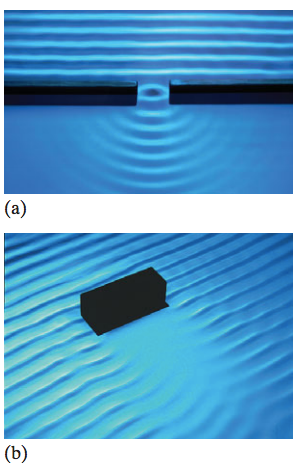
\includegraphics[width=.8 \linewidth]{diffraction_I.png}
        \caption{Diffraction des ondes.}
        \label{fig:diffraction_I}
    \end{minipage}
    \begin{minipage}{.5\textwidth}
        \centering
        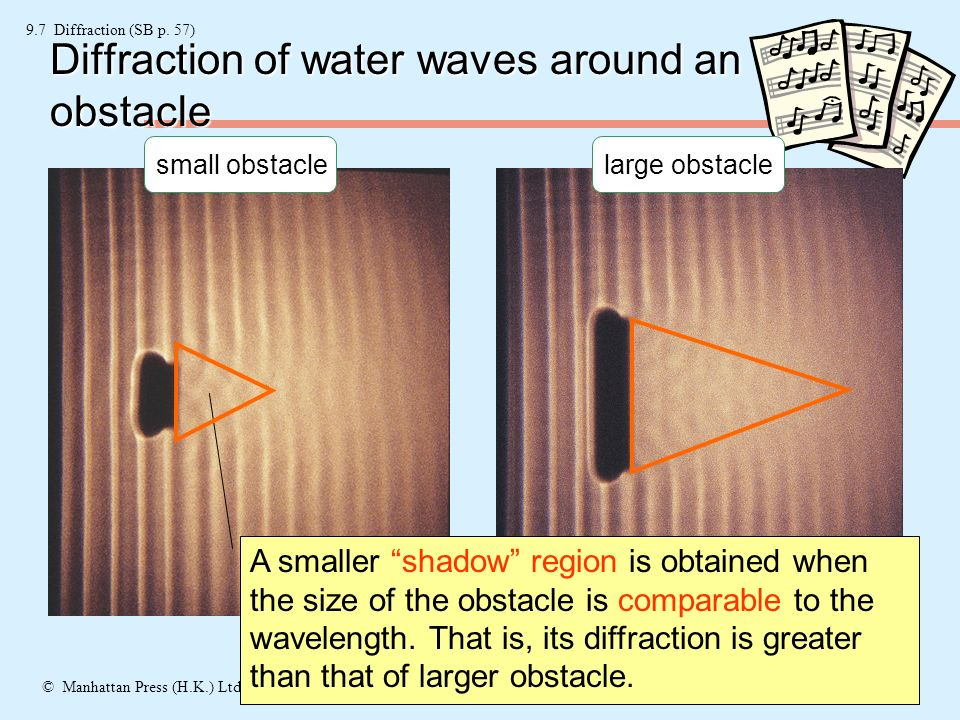
\includegraphics[width=.8 \linewidth]{diffraction_II.png}
        \caption{Taille de la zone d'ombre en fonction de la taille de l'obstacle.}
        \label{fig:diffraction_II}
    \end{minipage}
\end{figure}

\newpage

\subsection{Comprendre la diffraction : principe de Huygens}
Le principe de Huygens est simple et un lien clair peut être fait avec la résonance des oscillateurs :
\begin{encadre}
    \motcle{Principe de Huygens} : Lorsqu'une onde se propage, chaque élément de surface atteint par cette onde, se comporte comme une source secondaire qui émet des ondelettes sphériques appelées ondelettes d'Huygens.
\end{encadre}
L'oeil ne distingue pas ces ondelettes, mais uniquement leur enveloppe. Le front de l'onde à un instant \(t+\delta t\) se déduit du front de cette onde à l'instant \(t\), en considérant que l'enveloppe des ondes secondaires d'Huygens s'est propagée pendant l'intervalle de temps \(\delta t\), comme le montre la figure ci-dessous.

\begin{figure}[h]
    \centering
    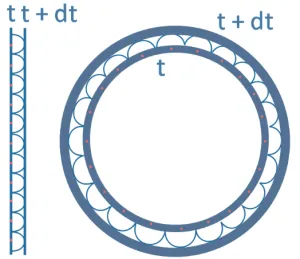
\includegraphics[width=.4\linewidth]{principe_huygens.png}
    \caption{Principe de Huygens (illustration et commentaire de \enquote{osez-reussir-en-physique.com})}
\end{figure}

Chaque point de part et d'autre d'un obstacle se comporte comme une source ponctuelle et un front d'onde se reforme dès lors derrière ceux-ci.
Lorsqu'une onde rencontre un obstacle complet comportant une fente étroite, celle-ci se comporte comme une source d'onde circulaire, ce phénomène est clairement visible dans l'illustration \ref{fig:diffraction_I} a et l'illustration \ref{fig:diffraction_IV}.

\begin{figure}[h]
    \begin{minipage}{.5\textwidth}
        \centering
        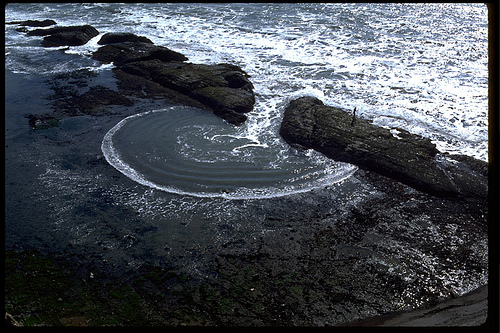
\includegraphics[width=.8\linewidth]{diffraction_IV.png}
        \caption{La diffraction à travers une fente étroite.}
        \label{fig:diffraction_IV}
    \end{minipage}
    \begin{minipage}{.5\textwidth}
        \centering
        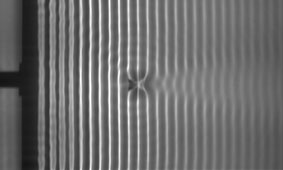
\includegraphics[width=.8\linewidth]{diffraction_III.png}
        \caption{La diffraction autour d'un obstacle de petite taille.}
        \label{fig:diffraction_III}
    \end{minipage}
\end{figure}

\subsection{Applications}

\begin{tcolorbox}[title=Ondes acoustiques]
    Le son est une onde dont la fréquence est comprise entre 20 Hz (fréquence la plus grave) et 20 000 Hz (fréquence la plus aiguë). La fréquence de référence est la note \enquote{la} (\(f=440[Hz]\)) à laquelle correspond une longueur d'onde de \(\lambda=0,77[m]\). Une longueur d'onde de \(1 [m]\) est associée aux sons de \(340[Hz]\). On réalise que les objets du quotidien (table, chaise, armoire, ouverture de porte, …) permettent une bonne diffraction des sons, c'est la raison pour laquelle ils se propagent bien dans l'ensemble des espaces que nous occupons.
\end{tcolorbox}

\begin{tcolorbox}[title=Écholocation]
    Lorsque les ondes diffractent bien autour d'un objet, elles s'y réfléchissent peu. La perception d'un corps grâce aux ondes qui s'y réfléchissent comme dans le cas du sonar, de l'écholocation (ondes sonores) ou du radar (ondes électromagnétiques) n'est donc possible que si la taille de l'objet recherché est plus grande que la longueur d'onde utilisée.
    La voix humaine crée en moyenne des ondes sonores comprises entre 125 et 210 Hertz, tandis qu'une chauve-souris génère des ondes comprises entre 15 000 et 150 000 Hz. Cet animal se nourri essentiellement d'insectes, comme les moustiques dont la taille est entre 0,5 et 1,5 centimètres.
    \begin{itemize}
        \item Calcule la taille des corps perceptibles par une chauffe-souris. Cela correspond-il à celle des insectes dont elles se nourrissent ?
    \end{itemize}
\end{tcolorbox}



\begin{tcolorbox}[title=Sonar]
    La fréquence d'émission d'un sonar est choisie en fonction de son utilisation. Les hautes fréquences (plusieurs dizaines ou centaines de kHz) sont rapidement absorbées par l'eau de mer (plusieurs centaines de mètres) mais, en revanche, permettent la détection de petits objets et peuvent ainsi réaliser de véritables images. Employées à une fréquence de 14 à 22 kilohertz durant la Seconde Guerre mondiale, elles sont donc, depuis, utilisées pour les sondeurs hydrographiques, les sonars de pêche, pour la recherche de mines, pour la détection de torpilles.
    Plus on descend en fréquence, plus les distances de détection sont grandes, mais on perd en finesse et les antennes deviennent très grandes et très lourdes. En pratique, les sonars actifs très basse fréquence ne descendent guère en dessous de 3 kHz. Les portées de détection n'excèdent pas quelques dizaines de kilomètres.
\end{tcolorbox}

\begin{figure}[h]
    \begin{minipage}{.5\textwidth}
        \centering
        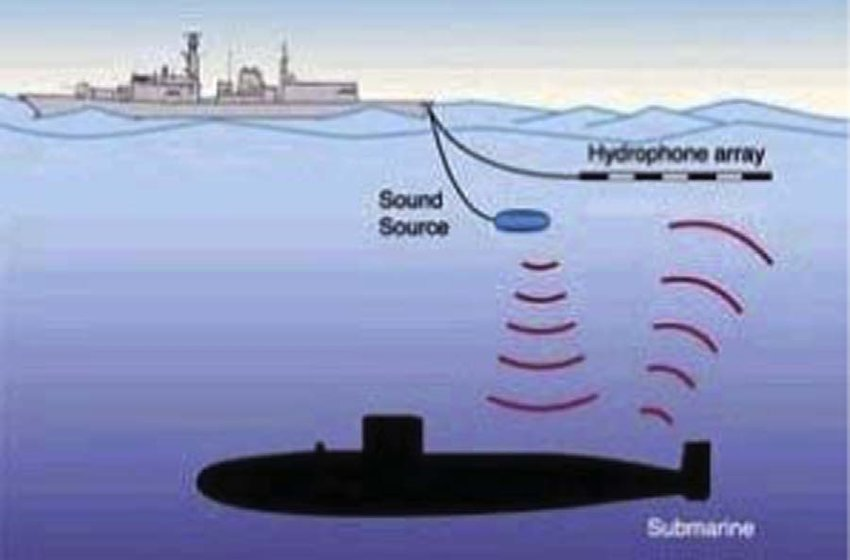
\includegraphics[width=.8\linewidth]{sonar.png}
        \caption{Le sonar}
    \end{minipage}
    \begin{minipage}{.5\textwidth}
        \centering
        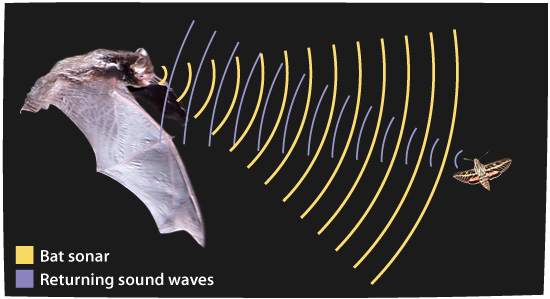
\includegraphics[width=.8\linewidth]{echolocation.png}
        \caption{L'écholocation chez les chauves-souris.}
    \end{minipage}
\end{figure}

\newpage

\section{Interférences}
Quand deux ondes atteignent simultanément un même point, elles vont agir dessus en respectant le \motcle{principe de superposition}. Si ces deux ondes sont de même amplitude, mais en opposition de phase, elles vont s'annuler mutuellement, on parle dans ce cas d'\motcle{interférences destructives}.
Si, au contraire, elles sont de même amplitude et en concordance de phase, elles vont se combiner et créer une \motcle{interférence constructive}.

\begin{figure}[h]
    \centering
    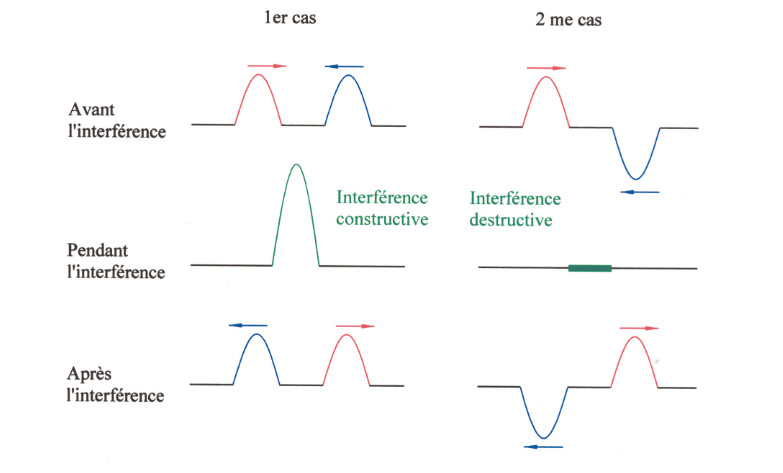
\includegraphics[width=.8\linewidth]{interference.png}
    \caption{Interférences constructives et destructives}
\end{figure}

\newpage

\section{Interférences entre deux sources ponctuelles}
Lorsque deux sources \textbf{en phase} et de \textbf{même amplitude} font vibrer le même milieu, chaque point de ce milieu va être affecté par les deux signaux. Il va donc y avoir une interférence des deux signaux en chaque point et une \motcle{figure d'interférence} va apparaître sur l'ensemble du milieu.

\begin{figure}[h]
    \centering
    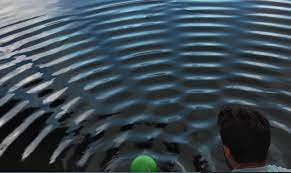
\includegraphics[width=\linewidth]{interference_deux_sources.png}
    \caption{Figure d'interférence pour deux sources en phase à la surface de l'eau.}
\end{figure}

\newpage

La figure ci-dessous représente un milieu soumis à l'influence de deux sources ponctuelles, en phase et de même amplitude. Repère sur cette figure les points correspondant aux interférences constructives et aux interférences destructives. Relie entre eux les points d'interférence constructive de manière à mettre en évidence les \motcle{lignes de tempête}, fais de même avec les interférences destructives pour mettre en évidence les \motcle{lignes de repos}.

\hfill \break

\begin{tikzpicture}[]
    \tkzDefPoints{-2/0/S1,2.5/0/S1_1UP,1.5/0/S1_2UP,2/0/S1_1DOWN,1/0/S1_2DOWN}
    \tkzDrawCircle[color=blue](S1,S1_1UP)
    \tkzDrawCircle[color=blue](S1,S1_2UP)
    \tkzDrawCircle[color=blue,style=dashed](S1,S1_1DOWN)
    \tkzDrawCircle[color=blue,style=dashed](S1,S1_2DOWN)

    \tkzDefPoints{2/0/S2,-2.5/0/S2_1UP,-1.5/0/S2_2UP,-2/0/S2_1DOWN,-1/0/S2_2DOWN}
    \tkzDrawCircle[color=red](S2,S2_1UP)
    \tkzDrawCircle[color=red](S2,S2_2UP)
    \tkzDrawCircle[color=red,style=dashed](S2,S2_1DOWN)
    \tkzDrawCircle[color=red,style=dashed](S2,S2_2DOWN)

    \tkzDrawPoint[color=blue,size=4pt](S1)
    \tkzDrawPoint[color=red,size=4pt](S2)
    \tkzLabelPoint(S1){\(S_1\)}
    \tkzLabelPoint(S2){\(S_2\)}

\end{tikzpicture}

\newpage

\begin{figure}[h]
    \centering
    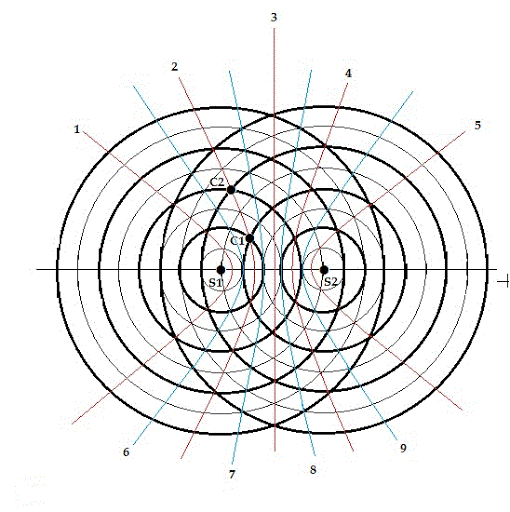
\includegraphics[width=\linewidth]{figure_interference.png}
    \caption{Figure d'interférence avec les lignes de tempête et de repos.}
\end{figure}

\newpage

\subsection{Condition d'interférences constructives ou destructives}
Dans la figure ci-dessous, les points rouges correspondent à des interférences constructives.
\begin{itemize}[label=\textbullet]
    \item Pour quelle raison y a-t-il des interférences constructives en ces points ?
          \pointilles{3}
\end{itemize}

\begin{figure}[h]
    \centering
    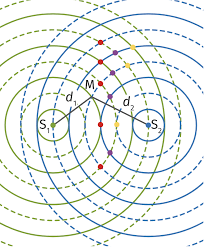
\includegraphics[width=.4\linewidth]{figure_interference_II.png}
    \caption{Figure d'interférence pour deux sources en phase.}
\end{figure}

La \motcle{différence de marche}, \(\lambda\), en un point correspond à la différence de distance entre ce point et chacune des deux sources : \(\delta _M=d_2 - d_1\). On peut donc dire qu'il y a une interférence constructive si la différence de marche vaut 0, mais ce n'est pas suffisant. En effet, il existe d'autres points présentant une interférence constructive, mais pour lesquels \(\delta \neq 0\), les points jaunes par exemple.

\newpage

\begin{itemize}[label=\textbullet]
    \item Quel doit être le déphasage entre les deux signaux arrivant sur un point jaune pour qu'ils interfèrent de manière constructive ?
          \pointilles{2}
    \item Que doit valoir la différence de marche en un point pour qu'il y ait une interférence constructive ?
          \pointilles{2}
\end{itemize}



Par un raisonnement similaire, on comprend qu'un point subit des interférences destructives si les signaux qui lui parviennent sont en opposition de phase, ce qui implique que la différence de marche vaut :

\begin{encadre}
    \motcle{Interférence destructive} : \(\delta = (2k+1) \frac{\lambda}{2} \ \ (k=0,1,2,3,...)\)
\end{encadre}

\begin{encadre}
    \motcle{Interférence constructive} : \(\delta = k \lambda \ \ (k=0,1,2,3,...)\)
\end{encadre}

\newpage

\begin{figure}[h!]
    \centering
    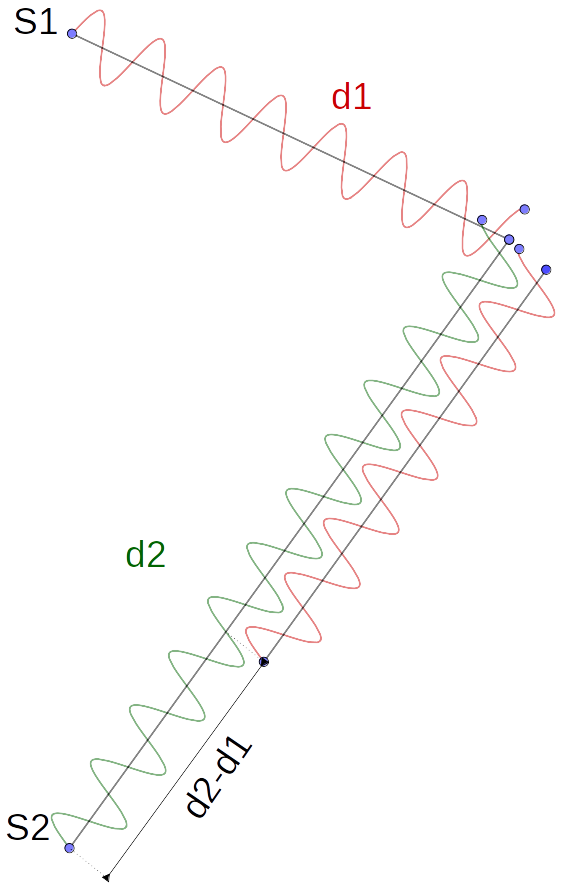
\includegraphics[width=.8\linewidth]{interference_difference_marche.png}
    \caption{La différence de marche vaut 4 lambda.}
\end{figure}

\newpage

\subsection{Étude mathématique des interférences}
Nous avons vu que l'élongation d'un point en fonction de sa distance à la source (\(x\)) et en fonction du temps (\(t\)) est donnée par : \(y_P (t) = A \cdot sin (\omega \cdot t- \frac{2 \pi  \cdot x}{\lambda})\).
Si un point se trouve à une distance \(x_1\) de la source \(S_1\) et une distance \(x_2\) de la source \(S_2\), alors, en vertu du principe de superposition, son élongation totale est donnée par :
\begin{equation}
    y_P (t) = A \cdot sin (\omega \cdot t- \frac{2 \pi  \cdot x_1}{\lambda}) + A \cdot sin (\omega \cdot t- \frac{2 \pi  \cdot x_2}{\lambda})
\end{equation}

On peut mettre l'amplitude en évidence pour avoir :
\begin{equation}
    y_P (t) = A \left \lbrace \cdot sin (\omega  \cdot t- \frac{2 \pi  \cdot x_1}{\lambda}) +  \cdot sin (\omega \cdot t- \frac{2 \pi  \cdot x_2}{\lambda}) \right \rbrace
\end{equation}

On sait que \(sin( a) + sin (b)=2 \cdot sin( \frac{a+b}{2}) \cdot cos(\frac{a-b}{2})\), donc :

\begin{equation}
    y_P (t) = A \cdot  sin \left \lbrace (\omega  \cdot t)- \frac{ \pi  \cdot (x_1+x_2)}{\lambda} \right \rbrace   \cdot cos \left \lbrace \frac{\pi}{\lambda}\cdot (x_1-x_2) \right \rbrace
\end{equation}

Cette équation est exactement celle de l'élongation d'un point dans le temps et dans l'espace, mais pour laquelle l'amplitude vaut \(A \cdot cos (\frac{\pi}{\lambda}\cdot (x_1-x_2) )\).

\subsubsection{Interférences destructives}
On sait que cette amplitude vaut \(0\) si \(cos \left \lbrace \frac{\pi}{\lambda}\cdot (x_1-x_2) \right \rbrace = 0\) , donc si :
\begin{equation}
    \frac{\pi}{\lambda}\cdot (x_1-x_2) = \frac{\pi}{2}+k \cdot \pi
\end{equation}

Ce qui revient à dire :
\begin{equation}
    (x_1-x_2) = \frac{\lambda}{2} \cdot (1+2\cdot k )
\end{equation}
Cette dernière équation correspond exactement à la condition pour laquelle il y a une interférence destructive.

\subsubsection{Interférences constructives}
En utilisant le même raisonnement, retrouve la condition de formation des interférences constructives.

\newpage

\section{Exercices}
\begin{exercise}
    Deux haut-parleurs sont distants de 1m et émettent un son à 1150Hz à une température de \(20^\circ C\). Une personne se trouve à 4m de l'un des hauts-parleurs, à quelle distance doit-elle se trouver du deuxième pour percevoir une interférence destructive ?
\end{exercise}
\begin{solution}\\
    \(k=1 \rightarrow x_2=4,296[m]\)\\
    \(k=-1 \rightarrow x_2=3,704[m]\)\\
    La deuxième réponse est \enquote{plus intéressante}, mais les deux sont acceptées.
\end{solution}

\begin{exercise}
    Deux haut-parleurs S1 et S2 distants de 6 émettent des ondes sonores en phase. Un point P se trouve à une distance de 8m de S1.
    \begin{enumerate}[a)]
        \item Pour quelle fréquence l'intensité en P est-elle maximale ?
        \item Pour quelle fréquence l'intensité en P est-elle minimale ?
    \end{enumerate}
    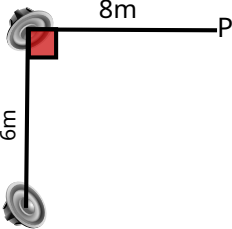
\includegraphics[width=.2\linewidth]{exercice_hauts_parleurs.png}
\end{exercise}
\begin{solution}
    \begin{enumerate}[a)]
        \item \(f=125,53[Hz]\)
        \item \(f=62,765[Hz]\)
    \end{enumerate}
\end{solution}

\begin{exercise}
    Deux haut-parleurs sont distants de 2,5m dans un local à \(20 ^ \circ C\). Une personne se tient à 3m de l'un des haut-parleurs et 3,5m de l'autre.
    \begin{enumerate}[a)]
        \item Quelle est la fréquence minimale qui provoque une interférence destructive en ce point ?
        \item Trouve deux autres fréquences qui provoque ce phénomène.
    \end{enumerate}
\end{exercise}
\begin{solution}
    \begin{enumerate}[a)]
        \item \(f_1=340[Hz]\)
        \item \(f_2=1020[Hz] ; f_3=1700[Hz]\)
    \end{enumerate}
    \(f_2\) et \(f_3\) correspondent à \(3 \cdot f_1\) et \(5 \cdot f_1\) puisque les interférences destructives sont obtenues avec les entiers impairs.
\end{solution}


\begin{exercise}
    Dans un local à \(20 ^\circ C\), une personne entend un son pur provenant de deux sources en phase et de même fréquence. Celle-ci est comprise entre 500 et 1000Hz. Le volume le plus élevé se trouve au point équidistant des deux sources. Afin de déterminer exactement la fréquence des sources, la personne se déplace et constate que le niveau est minimal lorsqu'elle est plus proche de 0,22m d'une des deux sources. Quelle est la fréquence du son ?
\end{exercise}
\begin{solution}
    Dans cette situation, on sait que : \(f=(2k+1) \cdot 772,727\).
    Pour \(k=1\), \(f=772,727[Hz]\). Cette fréquence est bien comprise entre 500 et 1000[Hz].
\end{solution}